% lint-skip: 未完成ステータス（figure/table caption 未対応，人手チェック時に解消予定）
\documentclass[../../main.tex]{subfiles}
\begin{document}

\begin{flushright}
  \footnotesize\textit{【自動文字起こし・要確認】}
\end{flushright}

{\bf [解答]} 時刻 $t$ での水深 $h$，水表面積 $S$ とおくと
\begin{align}
  V &= S \dfrac{dh}{dt} \cdots \text{\textcircled{1}} \\
  S &= V t + \pi a^2 \\
  &= \pi f(h)^2 \cdots \text{\textcircled{2}}
\end{align}

\begin{figure}[htbp]
  \centering
  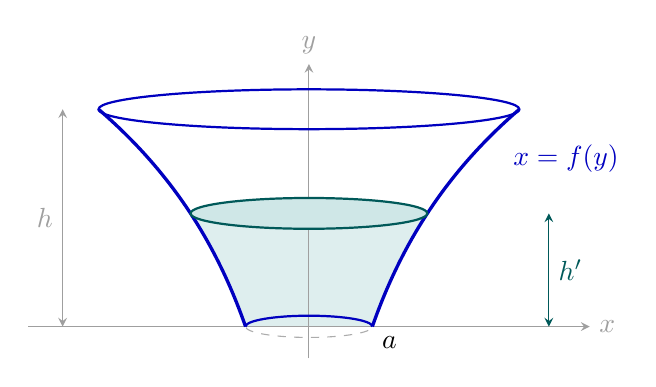
\begin{tikzpicture}[scale=1.15,>=stealth]
    % 図示用に a=0.7，容器の高さ h=2.4，水深 h'=1.25 とする。
    \fill[teal!13]
    plot[domain=0:1.25,samples=40] ({-0.7*exp(\x/2)},\x)
    -- plot[domain=1.25:0,samples=40] ({0.7*exp(\x/2)},\x) -- cycle;
    \draw[->,gray!75] (-3.1,0)--(3.1,0) node[right] {$x$};
    \draw[->,gray!75] (0,-0.35)--(0,2.9) node[above] {$y$};
    \draw[blue!75!black,very thick,domain=0:2.4,samples=80]
    plot ({0.7*exp(\x/2)},\x)
    plot ({-0.7*exp(\x/2)},\x);
    \draw[blue!75!black,thick] (0,2.4) ellipse[x radius=2.324,y radius=0.22];
    \draw[dashed,gray!65] (0,0) ellipse[x radius=0.7,y radius=0.12];
    \draw[blue!75!black,thick] (0.7,0)
    arc[start angle=0,end angle=180,x radius=0.7,y radius=0.12];
    \fill[teal!19] (0,1.25) ellipse[x radius=1.307,y radius=0.17];
    \draw[teal!70!black,thick] (0,1.25) ellipse[x radius=1.307,y radius=0.17];
    \draw[<->,gray!75] (-2.72,0)--(-2.72,2.4)
    node[midway,left] {$h$};
    \draw[<->,teal!70!black] (2.65,0)--(2.65,1.25)
    node[midway,right] {$h'$};
    \node[below right] at (0.7,0) {$a$};
    \node[blue!75!black,right] at (2.15,1.85) {$x=f(y)$};
  \end{tikzpicture}
  \caption{底面半径 $a$，高さ $h$ の容器と時刻 $t$ の水深 $h'$}
\end{figure}

\textcircled{2} と $f(y) > 0$ から
\[
  f(h) = \sqrt{a^2 + \dfrac{V}{\pi}t} \cdots \text{\textcircled{3}}
\]

\textcircled{2} を \textcircled{1} に代入，セパレして
\[
  \dfrac{V}{Vt + \pi a^2} dt = dh
\]
積分して，$C$ を定数とすると
\[
  \log \left( t + \dfrac{\pi}{V} a^2 \right) = h + C
\]
$t=0$ で $h=0$ だから，$C = \log \dfrac{\pi}{V} a^2$ なので，代入して
\begin{align}
  t &= e^h \cdot e^C - \dfrac{\pi}{V} a^2 \\
  &= \dfrac{\pi}{V} a^2 (e^h - 1) \cdots \text{\textcircled{4}}
\end{align}

$t=T$ で $h=h$ だから
\[
  T = \dfrac{\pi}{V} a^2 (e^h - 1) \quad \text{（終）}
\]

\textcircled{4} を \textcircled{3} に代入し，$h$ を $y$ でおきかえて
\[
  f(y) = a e^{\frac{y}{2}} \quad \text{（終）}
\]

\framebox{
  \begin{minipage}{0.9\textwidth}
    この時
    \[
      h' = \log \left( \dfrac{V t}{\pi a^2} + 1 \right), \quad S = \pi a^2 e^{h'} = \pi a^2 \left( \dfrac{V t}{\pi a^2} + 1 \right)
    \]
    より \textcircled{1} に代入
    \[
      V = (V t + \pi a^2) \cdot \dfrac{\pi a^2}{Vt + \pi a^2} \cdot \dfrac{V}{\pi a^2} = V
    \]
    $\implies$ あてそう
  \end{minipage}
}

\end{document}
